\section{Basics}

\subsection{Digital Signal Processing}

\subsubsection{Sampling and quantization}

If data from the real world should be processed in a digital system, it has to be sampled.
This process is has significant effects on the original signal so they have to be considered if
\ac{DSP} is taken seriously.

\subsubsection{Digital Filters}

Digital Filters are a huge field of digital signal processing. The most common filters are \ac{FIR}-filters.
The basic structure is a weighted shift register without feedback. The missing feedback is what makes
the \ac{FIR}-filter stable per construction.

In \autoref{fig:FIR-filter} the structure of a \ac{FIR}-filter is shown.

\begin{figure}[!h]
    \centering
    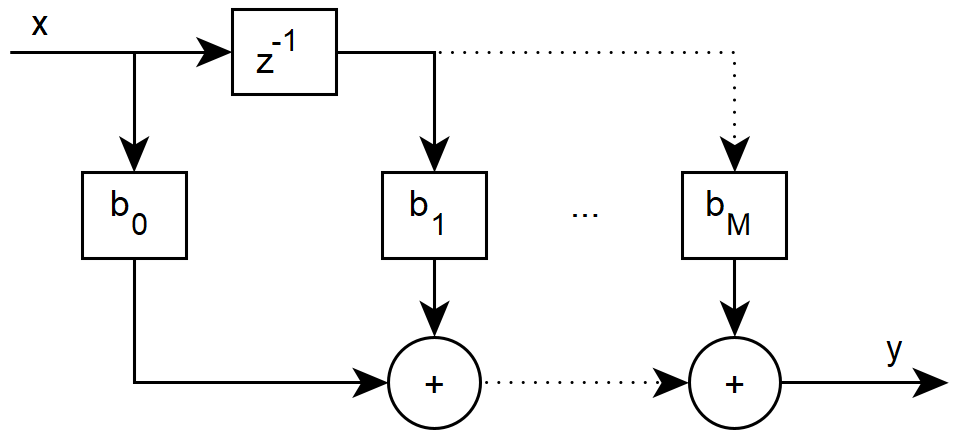
\includegraphics[width=7cm]{img/fir.png}
    \caption{Basic structure of a \ac{FIR}-filter \cite{meyer_signalverarbeitung}}
    \label{fig:FIR-filter}
\end{figure}

It can be seen that there are multiple components in this filter. The first component is the delay block,
which is described as $z^{-1}$. This block is responsible for adding a delay of one clock cycle to the input data.
Secondly, there are multiplikation blocks, noted as $b_M$. These blocks weight the input data and give the
result to an adder, which adds $M+1$ weighted and delayed signal samples. This sum is the output of an
\ac{FIR}-filter. It should be mentioned that the signal is transmitted without delay weighted with the coefficient
$b_0$.

The input signal is $x$, whereas the output is $y$. The order of this Filter is $M$ which means the amount of
filter taps or delay blocks.

A special case of the \ac{FIR}-filter is the moving average filter, at which all coefficients are $\frac{1}{M+1}$.

The whole system can be described with the difference equation in the time-domain (\autoref{eq:fir-difference-eq})

\begin{equation}
    y[n] = b_0 \cdot x[n] + b_1 \cdot x[n-1] + ... + b_M \cdot x[n-M]
    \label{eq:fir-difference-eq}
\end{equation},

or with the transfer function in the z-domain (\autoref{eq:fir-transfer-func})

\begin{equation}
    H(z) = \frac{Y(z)}{X(z)} = b_0 + b_1 \cdot z^{-1} + ... + b_M \cdot z^{-M}
    \label{eq:fir-transfer-func}
\end{equation}.

\subsection{Audio-Interfaces}

\subsubsection{Inter-Integrated Sound}

The \ac{I2S} protocol was developed by \textit{Philips} to share audio between \acp{IC}.
A similarity to the \ac{SPI} protocol can be recognized.

There are three signal lines:
\begin{itemize}
    \item SCK: Clock signal
    \item SD: Data signal
    \item WS: Word select, for ditinction between left and right channel
\end{itemize}
So the data is transmitted over the same signal line by time division multiplexing. 
To illsutrate the timing of the protocol the corresponding diagrams are shown in \autoref{fig:i2s-timing} \cite{nxp_i2s}.

\begin{figure}[!h]
    \centering
    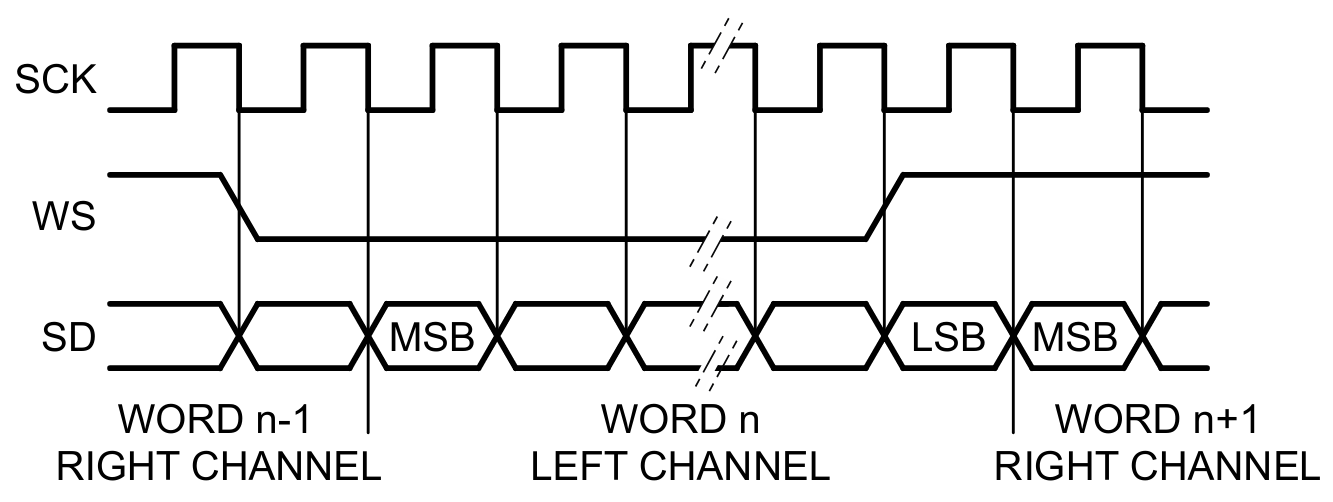
\includegraphics[width=10cm]{img/i2s_timing.png}
    \caption{Timing diagramm of the \ac{I2S} protocol \cite{nxp_i2s}}
    \label{fig:i2s-timing}
\end{figure}

The word length can vary between transmitter and receiver. That is why the \ac{MSB} is sent first in the standard 
configuration. Additionally the participants do not need to know the word length of the counterpart \cite{nxp_i2s}.

The wiring of this serial bus is possible in three basic configurations (shown in \autoref{fig:i2s-config}).
Thereby the master is always responsible for the SCK and the WS line.

\begin{figure}[!h]
    \centering
    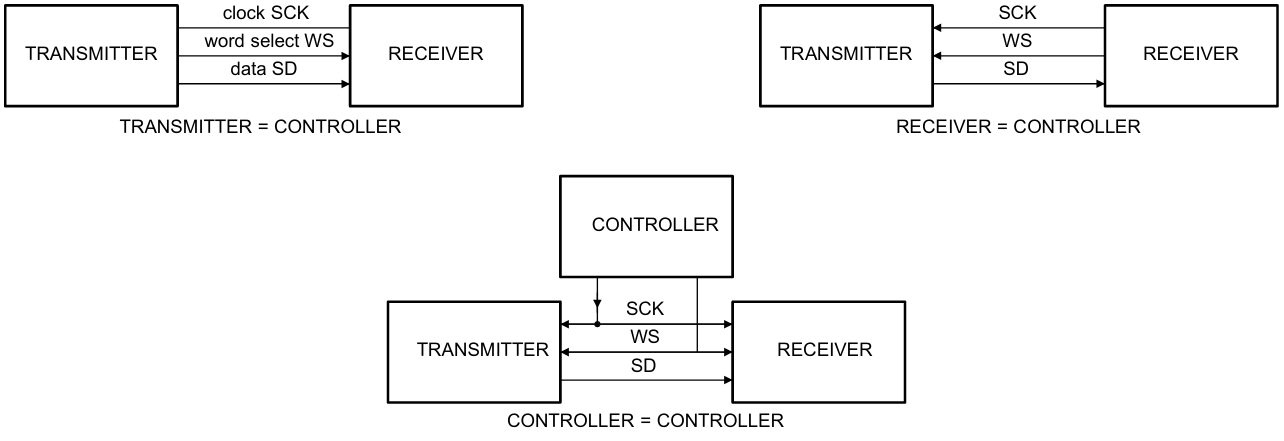
\includegraphics[width=14cm]{img/i2s_config.png}
    \caption{The three basic configurations of the \ac{I2S} protocol \cite{nxp_i2s}}
    \label{fig:i2s-config}
\end{figure}
